%%%%%%%%%%%%%%%%%%%%%%%%%%%%%%%%%%%%%%%%%%%%%%%%%%%%%%%%%%%%%%%
%
%                 LTI Library Developers Guide
%       Lehrstuhl fuer Technische Informatik, RWTH Aachen
%
%                         1999-2003
%
%%%%%%%%%%%%%%%%%%%%%%%%%%%%%%%%%%%%%%%%%%%%%%%%%%%%%%%%%%%%%%%

\documentclass[11pt,titlepage,a4paper]{scrreprt}
\usepackage[american]{babel}
\usepackage{varioref}
\usepackage{graphicx}
\usepackage{latexsym,fancyheadings}
\usepackage{here,named}
\usepackage{amsmath,amstext,amssymb}
\usepackage{array}
\usepackage{isolatin1}
\usepackage{fancybox}
\usepackage{multirow}
\usepackage{alltt}
\usepackage{makeidx} \makeindex
\usepackage{picinpar}
%
%%% check whether we are running pdflatex
\newif\ifpdf 
\ifx\pdfoutput\undefined 
\pdffalse % we are not running pdflatex 
\else 
\pdfoutput=1 % we are running pdflatex 
\pdfcompresslevel=9     % compression level for text and image;
\pdftrue 
\fi
%% For pdflatex
\ifpdf
\usepackage[pdftex,colorlinks,backref,pagebackref]{hyperref}
\else
\usepackage[backref,pagebackref]{hyperref}
\fi
%\usepackage{thumbpdf}


%% Seite Dimensionen f�r A4
\hoffset28mm
\voffset0mm
\evensidemargin0mm
\topmargin0mm
\headheight7mm
\headsep10mm
\textheight220mm
\textwidth130mm
\marginparsep3mm
\marginparwidth30mm
\marginparpush3mm
\footskip12mm

\parskip3mm
\parindent0mm

\pagestyle{fancy}

\lhead[\rm\thepage]{\sl\rightmark}
\rhead[\sl\leftmark]{
\includegraphics[width=2cm]{fig/lti-rwth}}

%%%%%%%%%%%%%%%%%%%%%%%%%%%%%%%%%%%%%%%%%%%%%%%%%%%%%%%%%%%%%%%
%
%    DOCUMENT
%
%%%%%%%%%%%%%%%%%%%%%%%%%%%%%%%%%%%%%%%%%%%%%%%%%%%%%%%%%%%%%%%
\begin{document}
\sloppy

%%%%%%%%%%%%%%%%%%%%%%%%%%%%%%%%%%%%%%%%%%%%%%%%%%%%%%%%%%%%%%%
%
%    Commands
%
%%%%%%%%%%%%%%%%%%%%%%%%%%%%%%%%%%%%%%%%%%%%%%%%%%%%%%%%%%%%%%%
\reversemarginpar

\newcommand{\marginlabel}[1]{%
  %\mbox{}\marginpar{\raggedleft#1}
  \makebox[0pt]{}\marginpar{\raggedleft#1}\ignorespaces}%

\newcommand{\lti}{\textsf{LTI\,}}
\newcommand{\rar}{$\rightarrow$}
\newcommand{\ltilib}{\textsf{LTI-Lib\,}}

\newcommand{\code}[1]{\texttt{#1}}
\newcommand{\zB}{z.\,B.}
\newcommand{\ZB}{Z.\,B.}
\newcommand{\ie}{i.\,e.}
\newcommand{\eg}{e.\,g.}
\newcommand{\Dh}{D.\,h.}
\newcommand{\product}[1]{\textsc{#1}}
\newcommand{\java}{\product{Java}}
\newcommand{\scheme}{\product{Scheme}}
\newcommand{\visualc}{\product{MS Visual C++}}
\newcommand{\cvs}{\product{cvs}}
\newcommand{\dqq}[1]{\glqq #1\grqq}
\newcommand{\sqq}[1]{\glq #1\grq}
\newcommand{\ltiurl}[1]{\underline{\textit{#1}}}

\newcommand{\cxx}{\textsf{ANSI C++\,}}
\newcommand{\stl}{\textsf{Standard Template Library\,}}

\newcommand{\button}[1]{\ovalbox{\footnotesize\rule{0pt}{1.8ex}\textsf{%
\textbf{#1}}}}
\newcommand{\radioButton}[1]{\footnotesize$\odot$~\textsf{\textbf{#1}}%
\normalsize}
\newcommand{\checkBox}[1]{\footnotesize$\Box$~\textsf{\textbf{#1}}%
\normalsize}
\newcommand{\txtfeld}[1]{\footnotesize\textsf{#1}\normalsize}
\newcommand{\typ}[1]{\texttt{#1}}
\newcommand{\icon}[1]{%
 \raisebox{-1ex}{\includegraphics[width=7mm]{#1}}%
}

\newcommand{\mbutton}[1]{\marginlabel{\button{#1}}}
\newcommand{\mradioButton}[1]{\marginlabel{\radioButton{#1}}}
\newcommand{\mcheckBox}[1]{\marginlabel{\checkBox{#1}}}
\newcommand{\micon}[1]{\marginlabel{\icon{#1}}}
\newcommand{\mtxtfeld}[1]{\marginlabel{\txtfeld{#1}}}
\newcommand{\mtyp}[1]{\marginlabel{\typ{#1}}}

%% Index %%

\newcommand{\inIndex}[1]{#1\index{#1}}
\newcommand{\boldIndex}[1]{#1\index{#1@\textbf{#1}}}

%%%%%%%%%%%%%%%%%%%%%%%%%%%%%%%%%%%%%%%%%%%%%%%%%%%%%%%%%%%%%%%
%
%       Titlepage
%
%%%%%%%%%%%%%%%%%%%%%%%%%%%%%%%%%%%%%%%%%%%%%%%%%%%%%%%%%%%%%%%

\begin{titlepage}

\newcommand{\HRule}{\rule{\linewidth}{1mm}}

\begin{tabular}{l l}
{\scriptsize\sc Rheinisch-Westf�lische Technische Hochschule Aachen}
& \multirow{3}{2mm}{
\includegraphics[width=44mm]{fig/lti-rwth}}\\
{\footnotesize\textbf{LEHRSTUHL F�R TECHISCHE INFORMATIK}} & \\
{\scriptsize\sc Prof.~Dr.-Ing.~Karl-Friedrich~Kraiss} & \\
\end{tabular}

\vspace{\stretch{1}}

\HRule
\vspace{8mm}

\begin{tabular}{l}
{\sffamily\bfseries\Huge LTI Image Processing Library}\\[1.5cm]
{\sffamily\bfseries\Huge Developer's Guide}\\[8mm]
\end{tabular}

\HRule

\vspace{\stretch{2}}

{\small{Version: 29.10.2003}}


\end{titlepage}

%%% Local Variables: 
%%% mode: latex
%%% TeX-master: "UsersGuide"
%%% End: 







\clearpage
\thispagestyle{empty}

\pagenumbering{roman}

%%%%%%%%%%%%%%%%%%%%%%%%%%%%%%%%%%%%%%%%%%%%%%%%%%%%%%%%%%%%%%%
%
%       Address      
%
%%%%%%%%%%%%%%%%%%%%%%%%%%%%%%%%%%%%%%%%%%%%%%%%%%%%%%%%%%%%%%%

\pagenumbering{roman}
\chapter*{}
\setcounter{page}{0}
\thispagestyle{empty}

\vspace*{\stretch{3}}

\mtxtfeld{Address}
\lti\ Computer Vision Library\newline
Lehrstuhl f�r Technische Informatik\newline
Ahornstr.\,55\newline
52074 Aachen

\mtxtfeld{E-Mail}
ltilib@techinfo.rwth-aachen.de

\mtxtfeld{WWW}
http://www.techinfo.rwth-aachen.de/ \newline
http://ltilib.sourceforge.net/

\mtxtfeld{Coordinators}Pablo Alvarado, Jochen Wickel,
                       Suat Akyol, Ulrich Canzler

\vspace{1cm}

{\small Der Lehrstuhl f�r Technische Informatik (\lti) und die Autoren
  �bernehmen weder implizit noch explizit Haftung irgendwelcher Art.  Der
  Benutzer tr�gt s�mtliche Risiken, die aus der Verwendung der Informationen
  dieses Dokuments resultieren.
  
  In keinem Fall kann der \lti\ f�r mittelbare oder unmittelbare, zuf�llige
  oder besondere Sch�den oder Folgesch�den, die aus einem Mangel der
  Dokumentation resultieren, haftbar gemacht werden.  Dies gilt auch, wenn auf
  die M�glichkeit eines solchen Schadens hingewiesen wurde.
  
  Der LTI beh�lt sich das Recht vor, dieses Dokument zu �berarbeiten und
  gelegentlich zu ver�ndern, ohne verpflichtet zu sein, zuvor irgendeine
  Person oder Organisation �ber solch eine �berarbeitung oder �nderung zu
  unterrichten.%
}

\vspace{1cm}

{\small The Chair of Technical Computer Science (\lti) and the authors assume
  no responsibility for errors or omissions, or for damages resulting from the
  use of the information contained herein.
  
  The \lti\ reserve the right to change the contents of this document at any
  time without notice.
}

\vspace{1cm}

All terms mentioned in this document that are known to be trademarks or
service marks have been appropriately capitalized.  Use of a term in this
document should not be regarded as affecting the validity of any trademark or
service mark.


\clearpage

\thispagestyle{empty}

%%% Local Variables: 
%%% mode: latex
%%% TeX-master: "DevelopersGuide"
%%% End: 









%%%%%%%%%%%%%%%%%%%%%%%%%%%%%%%%%%%%%%%%%%%%%%%%%%%%%%%%%%%%%%%
%
%       Contents
%
%%%%%%%%%%%%%%%%%%%%%%%%%%%%%%%%%%%%%%%%%%%%%%%%%%%%%%%%%%%%%%%

\setcounter{tocdepth}{2}
\setcounter{secnumdepth}{2}

\tableofcontents

%%%%%%%%%%%%%%%%%%%%%%%%%%%%%%%%%%%%%%%%%%%%%%%%%%%%%%%%%%%%%%%
%
%       Chapters
%
%%%%%%%%%%%%%%%%%%%%%%%%%%%%%%%%%%%%%%%%%%%%%%%%%%%%%%%%%%%%%%%

\chapter*{License}

Copyright (C) 1998, 1999, 2000, 2001, 2002 

Lehrstuhl fuer Technische Informatik (LTI), RWTH-Aachen, Germany
 
This documentation is part of the LTI-Computer Vision Library (\ltilib)

The \ltilib\ is free software; you can redistribute it and/or modify it under
the terms of the GNU Lesser General Public License (LGPL) as published by the
Free Software Foundation; either version 2.1 of the License, or (at your
option) any later version.

The \ltilib\ is distributed in the hope that it will be useful, but WITHOUT
ANY WARRANTY; without even the implied warranty of MERCHANTABILITY or FITNESS
FOR A PARTICULAR PURPOSE.  See the GNU Lesser General Public License for more
details.

You should have received a copy of the GNU Lesser General Public License along
with the \ltilib\; see the file LICENSE.  If not, write to the Free Software
Foundation, Inc., 59 Temple Place - Suite 330, Boston, MA 02111-1307, USA.

More information can be found in the Internet:

\url{http://www.gnu.org/licenses/licenses.html}

%%% Local Variables:
%%% mode: latex
%%% TeX-master: "DevelopersGuide"
%%% End: 

\chapter{Introduction}
\label{chap:introduction}
\pagenumbering{arabic}

The \inIndex{\ltilib}\ encloses a collection of algorithms and data structures
commonly used in image processing and computer vision applications, developed
at the Chair of Technical Computer Science (in German \emph{\textbf{L}ehrstuhl
fuer \textbf{T}echnische \textbf{I}nformatik} (\lti) ), RWTH Aachen
University.  It is written in C++ in order to allow both object oriented
programming as well as efficient resulting code.
%
Its main goal is to provide a system independent library, adhering as
closely as possible to the \cxx\ standards.  It is intended to work on
different operating systems, but it specially supports for \product{Linux/gcc}
and \product{MS WindowsNT}/\visualc\ systems.

\section{History}

In the last years, several research groups at the \lti have worked on
different applications in the field of computer vision.  
%
Before 1999, all projects using image processing algorithms (Sign Language
Recognition, Mobile Service Robots and Visual Information Retrieval) developed
their own software and applications independently.  Two typical
problems arose:

\begin{enumerate}
\item work efforts were being wasted due to unnecessary code duplication
\item reusing code was difficult or even impossible due to the lack for
  standardized interfaces.
\end{enumerate}

These reasons forced the design of an internal library, which has been now
used and extended for a while in all groups at the \lti.  The choice to
develop a new library was based on several factors:

First, we required a C++ library that followed a consistent object-oriented
concept.  This was intended to simplify the software development, enhancement
and maintainability.  Many libraries were implemented in C, or in a C-like C++
that was not appropriate to enhance or to adapt to our requirements.  Others
lacked a fundamental concept that could be employed in further developments.

Second, the library should provide not only algorithms for image processing,
but also for mathematical and statistical tasks, allowing a flexible
interchange of data between all modules.  Many existent libraries did not
fulfill these requirements.

Third, some of the regarded libraries were not maintained any more, some had
no documentation at all.  Commercial libraries were well documented and
had nifty rapid prototyping tools, but due to a ``closed source'' concept, it
would be impossible to enhance or to change existing algorithms without
reimplementing them.  This last point is unacceptable for research purposes.

Fourth, very powerful and widespread tools used in research (like
\product{Matlab}) can be used to search for solutions of relatively small
problems, but they showed to be usually too slow for more complex applications
or complete prototypes involving the whole scope from image acquisition and
processing to feature extraction and classification.  We usually required
implementations that can run in real-time or that involve huge amounts of
data.

The creation of a new library at the \lti\ was not a start-from-scratch
project, due to the existence of previous code and sufficient expertise from
all research projects.  At the beginning, an interface was specified and the
most important algorithms were adapted to it.  The \ltilib\ has grown to more
than 750 classes (more than 350000 lines), covering image processing,
mathematics, statistics, neural networks, hardware interfaces, etc. with all
objects following the same concept.

\index{advantages} The use of \emph{one} library saves development time, which
otherwise would be required in re-implementing commonly used algorithms.  This
time can now be invested in the development of new solutions or optimizing
already existing ones.  This way, not only one developers group will
benefit from improvements, but all the users of the library.
%
Its use increases also the code readability, due to the fact
that all, complex and simple tasks, will now follow general known
specifications.  Further development or maintenance are therefore easier.

The following chapters explain the concepts behind the \ltilib\ interface, and
presents all specifications required in the program coding.

%%% Local Variables: 
%%% mode: latex
%%% TeX-master: "DevelopersGuide"
%%% End: 











\chapter{LTI-Lib Architecture}
\label{chap:architecture}

The \ltilib\ is easy to use due to the specification of a consistent
programming interface for all classes.  The preservation of this consistency
is partially achieved through the use of the \product{PERL}-script
\code{ltiGenerator}.  Based on a few rudimentary data provided by the
programmer (like class name and parent class) this script builds some template
files, containing all standard definitions.  After that, only the
functionality needs to be implemented.  This chapter explains all basic
concepts required to understand the meaning of this classes.

\section{Functors, parameters and states}

Most algorithms require \emph{parameters}, i.\,e.\ user defined values that
modify its behavior.  For example, the file name is a parameter of an image
loader class, or the size of a filter kernel is a parameter of a convolution
algorithm.
%
All algorithms in the \ltilib\ are encapsulated in so called \index{functor}
functor-classes.  They always enclose a class called \code{parameters}, that
can be explicitely declared or just inherited from the parent class.

This means, when you use the \ltilib\ you do not call some functions or class
methods with lots of confusing arguments, some meaning input data, others the
output data, and additionally a long list of parameters.  A default parameters
object is usually stored within the functor class, and all methods that provide
the algorithmic functionality expect from the user only the input data and the
output objects where the results are going to be written.  You can of course
change the used parameters to fit the functor's functionality to your needs.

The parameters of a functor have to be distinguished from its state, which
consists of all those attributes of the class that are computed during the
execution of the algorithm, but are not directly provided or required by the
user.  For the \emph{Motion History Images}(\code{lti::temporalTemplates}) for
example, the last presented image must be kept in order to compute the next
iteration.  This image is not a parameter, but a part of the functor's state.
These concepts are shown in Fig.~\ref{fig:functor}.

\begin{figure}[htbp]
  \begin{center}
    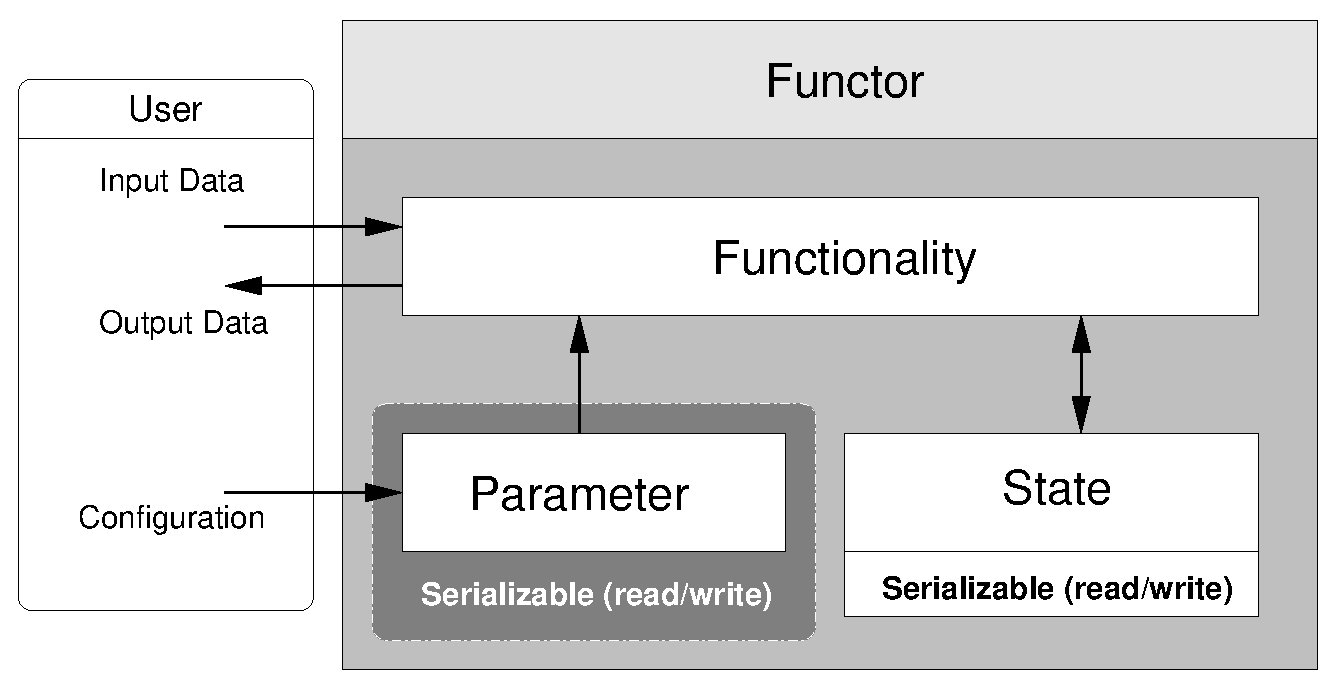
\includegraphics[width=10cm]{fig/functor}
    \caption{Architecture of a functor.  The user can change the behavior of
      the functor through the parameters.  The functor can also have a state,
      that eventually (like the parameters) can also be saved.}
    \label{fig:functor}
  \end{center}
\end{figure}


There are several reasons for an independent parameters class.  You can create
several instances with different value sets and change at once the
functionality of your functor with a simple \code{setParameters()}.  You can
load and save your parameters object in a file, or can give it to a graphical
user interface where the user can choose between several values.

The parameters contain values directly specified by the user and they should
not be modified by the functor.  If a programmer thinks his/her
algorithm must change a parameter, this is just a sign that this parameter
should be copied somewhere else at the beginning of the algorithm, like a
local variable or a state variable (an attribute of the functor class).

An usual question is: why do I need to call the method \code{getParameters()}
to get the parameters instance? would it not be faster if each functor-class
had its own parameters instance that it could use directly?

\begin{figure}[htbp]
  \begin{center}
    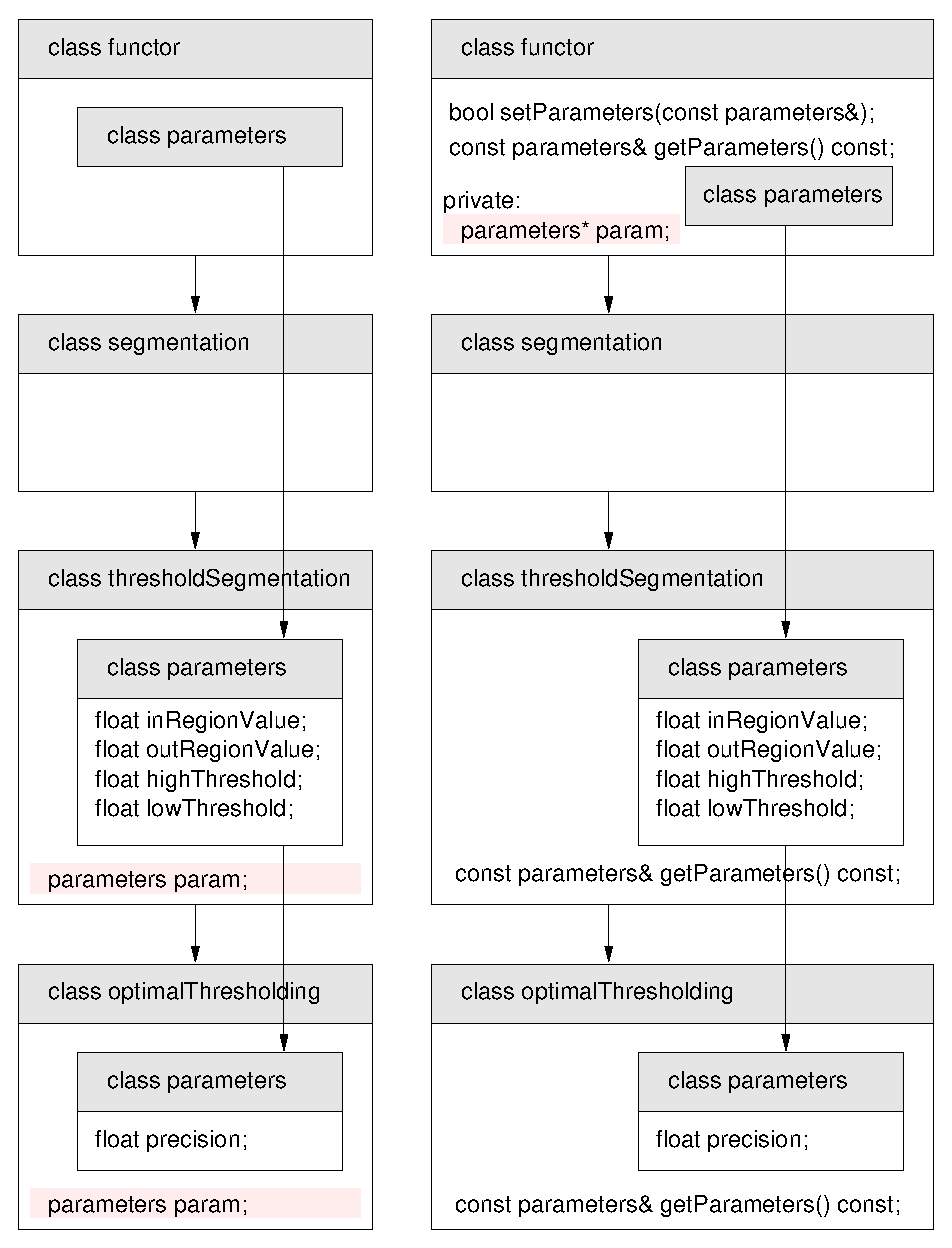
\includegraphics[height=16cm]{fig/paramhier}
    \caption{Example for the functor hierarchy: on the left side the naive way
      with several parameters-class instances (this implies a very inefficient
      memory management).  On the left side the \ltilib\ way with just one
      parameters-class instance.}
    \label{fig:paramhier}
  \end{center} 
\end{figure}

The answer relies partially on memory management issues.  It would be very
expensive if all classes in the functor hierarchy would have their own instance
of the parameters, because all inherited parameter attributes would be present
several times.  With the functor hierarchy shown on the left side of
Fig.~\ref{fig:paramhier}  an instance of the functor
\code{lti::optimalThresholding} would have two parameter objects: the one of
its own with five attributes (\code{precision} and the five attributes of the
parent class) and the parameters-instance of \code{lti::thresholdSegmentation}
with its four attributes.  In other words, the four attributes of the parent
class are present twice!

To avoid this problem, there exist just one instance of the parameters in the
functor class.  Each class casts this instance to the proper parameters type
using the overloaded method \code{getParameters()}.

Another important reason for the use of just one parameters-instance in the
functor class appears when the inherited class calls methods of the parent
classes, the later ones could not see the proper parameters-instance but only
the own one, which could contain other values than those specified by the
user.

The functionality of a functor is always accessed by its methods
\code{apply}.  They expect input data, (usually constant references to objects
like matrices or images), and references to output objects (references to
containers where the result is written).  Functors also provide the so
called \emph{shortcut}-methods that simplify the use of specific
functionality.  For example, to load an image file, the image loaders provide
the shortcut \code{load} that expects the file name and the image where the
result should be left.  Otherwise, you would require to create a parameters
object, set there the filename, give this parameters-instance to the functor,
and at last call the apply method:

{\small
\begin{alltt}
  // an image
  lti::image img;

  // functor to load images in Windows BMP format:
  lti::loadBMP loader;

  // parameters for the loader
  lti::loadBMP::parameters loaderParam;

  // the file to load
  loaderParam.filename = "testimage.bmp";

  // load the image into img
  loader.setParameters(loaderParam);
  loader.apply(img); // load the image!

\end{alltt}
}

It is much easier and comfortable to employ following shortcut:

{\small
\begin{alltt}
   // an image
  lti::image img;

  // functor to load images with Windows BMP format:
  lti::loadBMP loader;

  // load an image
  loader.load("testimage.bmp",img);
    
\end{alltt}
}

All functors must nevertheless provide an interface based on a
\code{parameters}-object and \code{apply}-methods, in order to provide complex
higher-level applications a uniform way to access the functionality of the
functor.

Within the apply methods you can avoid an unnecessary copy of the
parameters-instance getting a constant reference to them, for example:

{\small
\begin{alltt}
/*
 * apply method for myFunctor. Do something on the src vector and
 * leave the result in the dest vector.
 * @param src the input vector
 * @param dest the output vector
 * @return true if successful, false otherwise
 */
 myFunctor::apply(const vector<double>& src, vector<double>& dest) \{
   
   // Get a const reference to the functor parameters
   const parameters\& param = getParameters();

   // use the parameters to do something, assuming you have
   // an attribute called "justCopy" in the parameters
   if (param.justCopy) \{
     dest.copy(src)
   \} else \{
     // do something else ...
   \}

   return true;
 \}
\end{alltt}
}

Please remember, the parameters should never be changed within the
\code{apply}-methods:     

{\small
\begin{alltt}
bool myFunctor::apply(...) \{

  ...

  const parameters& param = getParameters();

  param.justCopy = false;  // is not possible, param is const!
  
  // you should NEVER EVER do something like this:
  const_cast<parameters*>(&param)->justCopy = false;

  // do something like:
  
  // a local copy of the parameters' attribute
  bool justCopy(param.justCopy);

  justCopy = false; // the local copy may be changed!

  ...
\}
\end{alltt}
}

There exist just one \code{getParameters}-method and it returns a
\emph{constant} reference to the parameters-instance, this due to the fact
that the parameters must not be changed by the functor.

As mentioned above, the functor may provide some \emph{shortcuts}
that allow changing specific parameter values.  These methods, of course,
should not be called within the \code{apply} methods.

Besides the parameters, a functor may have a state, where it stores
information irrelevant for the user but necessary for later computations.
An example for a functor with separated state and parameters is the
\code{lti::principalComponents} object.  Here you find a parameter
\code{autoDim} which indicates that another parameter
\code{resultDim} should be detected automatically.  In the \code{apply} method
this last value is not changed.  The computed transformation matrix is part of
the functor state, which can be used later to transform other vectors.  This
matrix is not something that the user can give directly, but can be saved and
loaded with other parts of the functor's state (this is done when you
load or save the whole functor).

All functors with a state relevant for later computations can be saved and
loaded, i.\,e.\ they overload the methods \code{read} and \code{write}.

\section{Input and Output in the \ltilib}

Serializable objects in the \ltilib (\ie\ objects that can be written or read
from disk) never directly use \code{std::fstream} objects.  The main reason is
that we need to provide a way to support different file formats at the same
time.  The desired file format is determined through a so called
\code{lti::ioHandler}.  At this time there are two file formats.  A Lisp-like
one writes or reads ASCII strings in or from a given stream, where
different scopes are delimited with parenthesis.  A binary format 
produces shorter files and is faster to be read or written, but can not be
edited by hand.

A uniform way to load or save \ltilib-objects and internal types (\code{int},
\code{float}, \code{double}, \code{std::string}, etc.) is provided through
four global functions that passes them properly to a given \code{ioHandler}.
These are:

{\small
\begin{alltt}
  bool lti::write(ioHandler& handler, 
                  const T& data);

  bool lti::read(ioHandler& handler,
                 T& data);


  bool lti::write(ioHandler& handler, 
                  const std::string& name,
                  const T& data,
                  const bool complete=true);

  bool lti::read(ioHandler& handler, 
                 const std::string& name,
                 T& data,
                 const bool complete=true);
\end{alltt}
}

The first two functions write or read the contents of an object of type
\code{T} in or from the given \code{ioHandler}.  The third and fourth methods
write the data together with a name that identifies this object.  To read
the data, the given name must match the one used as the data was saved.

With a handler of type \code{lti::lispStreamHandler} following lines
{\small
\begin{alltt}
  lti::write(handler,"a",5);
  lti::write(handler,"b",9);
\end{alltt}
}

produce the following output in the output stream associated with the handler:
{\small
  \begin{alltt}
    (a 5)
    (b 9)
  \end{alltt}
}

The parenthesis around each line can be left out if the fourth parameter of
the functions (\code{complete}) is set to \code{false}.  Note that the default
value for this parameter is \code{true}.

The \code{lti::lispStreamHandler} can find an object using its name:
{\small
\begin{alltt}
  int x,y;
  lti::read(handler,"a",x);
  lti::read(handler,"b",y);
\end{alltt}
}

After these lines it applies \code{x==5} and \code{y==9}.  Some
\code{ioHandler} (for example \code{binaryStreamHandler}) require that the
read order matches the one used when writing.  If this is not true, the read
methods will return \code{false}.  Other \code{ioHandler} (like
\code{lispStreamHandler}) search for the data using the given name as key, so
that you can use a different reading order.  Following lines would also result
in \code{x==5} and \code{y==9}:

{\small
\begin{alltt}
  int x,y;
  lti::read(handler,"b",y);
  lti::read(handler,"a",x);
\end{alltt}
}

The \code{ioHandler} concept makes it possible to define new file formats
\emph{without} requiring to reimplement all read and write methods of the
\ltilib-classes.  Due to the fact that the read and write methods use a
rigorous syntax, it is also relative simple to parse the files.

Please note that the variables used in the previous examples could also have
any other type defined in the \ltilib.   All numerical standard types
(\code{int}, \code{double}, etc.), the Standard Template Library (STL) types 
\code{std::vector}, \code{std::list} and \code{std::map} (if you include the
file ``\code{ltiSTLIoInterface.h}'') and the most \ltilib\ functors,
parameters and data structures can be serialized.

\subsection{Example}

How can I save and load some parameters in my program?

{\small
\begin{alltt}

  // ltilib functors and their parameters
  lti::csPresegmentation segmentor;
  lti::csPresegmentation::parameters segParam;

  lti::orientationFeature orientor;
  lti::orientationFeature orientParam;

  // ... initialize the parameters ...

  // how can we write the parameters in a file named "param.txt"?
  lti::lispStreamHandler handler;  // the stream handler
  std::ofstream out("param.txt");  // the std::fstream used

  // if the output stream is ok, write the data
  if (out) \{
    // the handler have to write the data using the stream "out":
    handler.use(out);
    
    // write the parameters:
    lti::write(handler,"orientParam",orientParam); 
    lti::write(handler,"segmentParam",segParam);
    lti::write(handler,"anInteger",5);
  \}


  // how can we read the data from "param.txt"?
  std::ifstream in("param.txt");

  if (in) \{
    int x;

    handler.use(in);
    
    // read the data
    lti::read(handler,"orientParam",orientParam); 
    lti::read(handler,"segmentParam",segParam);
    lti::read(handler,"anInteger",x);
  \}
\end{alltt}
}

\section{Visualization Classes}

Not everything in an image processing or computer vision library can be
considered as functor.  Examples for this are the so called drawing and
visualization objects.

Drawing objects does not execute one algorithm.  They provide different tools
to draw simple geometric constructs on images or other output media.  To use a
drawing object you need to provide it with your \emph{canvas}, \ie\ you need to
specify the image where you want to draw.  This is done with the method
\code{use}.  After that, you can choose the color you want to use with the
method \code{setColor}.  All lines, circles or points you draw after this,
will be painted using the given color.

Following example draws a circle and a line on a color image:

{\small
\begin{alltt}
  lti::image img(256,256);  // our canvas

  lti::draw<rgbPixel> drawing;  // drawing tool
  
  drawing.use(img);                      // where should "drawing" paint on?
  drawing.setColor(lti::Blue);           // Blue color
  drawing.circle(lti::point(128,128),
              20,true));              // filled circle, radius 20
  drawing.setColor(lti::Red);            // Red color
  drawing.line(10,10,128,128);           // A red line
\end{alltt}
}

Viewer objects do not modify any data, but provide simple ways to
visualize them.  The presentation of the data persists as long as the viewer
object exists.

You can show the previously drawn image with following code:

{\small
\begin{alltt}
  lti::viewer viewer("This is art");  // our viewer object
  viewer.show(canvas);                // show our master piece
  getchar();                          // just wait 
\end{alltt}
}

\section{Classifiers}

Other important object classes that do not fit into the functor paradigm are
the classifiers.  They provide methods to learn from data and to use the
learned information to analyze new data.  There are different interfaces for
the supervised and unsupervised classifiers.  Both types can be categorized
into instance classifiers that learn single vectors (like traditional neural
networks) and sequence classifiers that also considered time aspects (like the
Hidden Markov Models).

In the \ltilib\ all classifiers deliver the results using the same data
structures \code{lti::classifier::outputVector}, so that the processing of
their results does not depend on the specific classifier used.

%%% Local Variables: 
%%% mode: latex
%%% TeX-master: "DevelopersGuide"
%%% End: 

\newcommand{\staticcast}{\code{static\_cast}}

\chapter{C++ Programming Style Guide}

The Programming Style Guide provides several necessary rules to keep a clean
and consistent development environment.  Through this rules it is easier for a
developer to find his way in the code, even if he is not the original author.

The main goal of the \ltilib\ is to provide a system independent library,
which follows as much as possible the ANSI standards.  The system should work
on different \product{Unix}-Platforms and on \product{Windows}, but it is
specially maintained for \product{Linux} and \product{WindowsNT} machines.  To
achieve this, strict programming discipline is required.  System dependent
``tricks'' are not allowed.

In those cases where is not possible to write system independent code (for
example, due to direct hardware access), the platform dependent parts must be
isolated in the smallest possible units.  An access class have to be
specified, which provides access to all special supported operations.  No
direct platform dependent access is allowed.

\section{Organisation of the data}

\subsection{Version control}

\index{version control|see{CVS}} All code files will be administrated using a
\inIndex{CVS}-database.  The repository will be on the CVS-Server.  A few
hints to use CVS are available.  There are many graphic front-ends to simplify
the use of this version control system, like \product{WinCVS} for
\product{Windows} (\url{http://www.wincvs.org/}) or \product{Cervisia} for
\product{Linux/KDE} (\url{http://cervisia.sourceforge.net/}).

Each developer should not forget to comment its changes when committing into
the repository.  To avoid confusion, he/she should try to get only one copy of
the \ltilib\ (for the CVS-Server there is no problem, but some developers have
lose some work because they did changes somewhere else...).

\subsection{\inIndex{File conventions}}

\index{filenames|see{file conventions}}
\begin{itemize}
\item Header files have always the extention \code{.h}.
\item Source files have always the extention \code{.cpp}.
\item Different words in a file name are written together, and each word
  (except the first one) must begin with an uppercase letter.  The first word
  must be \code{lti}.  Examples: \code{ltiFunctor.h} \code{ltiLinearFilter.h}
\item Files which contain implementation for inline or template methods or
  functions must be clearly denoted with \code{\_template} or
  \code{\_inline}.  For example \code{ltiMatrix\_template.h}
  \index{\code{template}} (see also section \ref{ssec:templates}).
\end{itemize}

\section{Tools}

\subsection{Debugging}

Search your \emph{bugs} with a \inIndex{Debugger}.  On \product{Windows NT}
you can use the \visualc-Debugger.  On \product{Linux} there are many
front-ends for the GNU-Debugger gdb, like \product{xxgdb}, \product{kdbg} and
\product{ddd}.  A class must work without problems before it is integrated in
the rest of the \ltilib.  To test your new functors, you can use the
\code{tester} project provided with the library.

Other commercial products like \product{Purify} can help searching for memory
problems like memory leaks or outer-bounds access of arrays.

If a program crashes, it usually helps to catch the \code{lti::exception}s and
ask their content with the method \code{what()}) (see also section
\ref{sssec:exception}).  It also helps to check if the called \code{apply()}
or other functor methods return \code{false}, and in that case the cause of
the problem can be checked with the \code{getStatusString()} method.

\subsection{Optimization}

Try to implement efficient code, but in a way that it remains
maintainable.  You can use \product{gprof}, \product{valgrind} or the
\visualc\ profilers to detect the critical parts of your code, which
may require special attention by optimization.

\section{General programming conventions}

\subsection{Preamble}

Each violation to the programming conventions must be documented.  It is not
always possible to respect all conventions.  There are even cases where they
are contradictory and following one will violate another.  Each case has to
be studied separately to decide which solution makes more sense.  Discuss
these cases with other \ltilib\ developers.

\subsection{Name conventions}

The names of classes, methods, functions and variables must always make sense.
They all must be in English.  Comments must be also in English.  These way,
your code can be understand all around the world.

\section{C++-Programming}

C++ was chosen as the main language for the \ltilib\ because it is possible to
efficiently implement time and memory intensive algorithms (which are common
in computer vision) without sacrificing code maintainability and using modern
object oriented approaches.  It is also important to know where to look up for
information.  There are two helpful books \index{C++ Books}: \cite{primer} is
a very good introductory book for C++ and \cite{stroustrup}, in which almost
everything about C++ can be found, even if it is sometimes difficult to find.

\subsection{File organization}

\newcommand{\thelog}{Id}

\begin{itemize}
\item each file with source code begins with a comment including information
  about the file, like licence conditions, filename, authors, creation date,
  etc.  If a special comment is present (see \code{\$\thelog} in the next
  example), \cvs\ automatically enters some information in the file history:

{\small
\begin{alltt}
/*--------------------------------------------------------------
 * project ....: LTI Digital Image/Signal Processing Library
 * file .......: ltiThread.h
 * authors ....: Thomas Rusert
 * organization: LTI, RWTH Aachen
 * creation ...: 03.11.99
 * revisions ..: $\thelog: ltiThread.h,v 1.6 2003/02/17 07:17:01 author Exp $
 */
\end{alltt}
}

\item you should avoid multiple inclusion of header files:
  \index{\code{include}}
\begin{verbatim}
#ifndef HEADER_FILE_NAME_H
#define HEADER_FILE_NAME_H
...
#endif
\end{verbatim}

\item each class definition required in other header or implementation files,
  must have its own header file.
\item header files of the \ltilib\ must be included with
  \verb+#include "filename"+, system files with
  \verb+#include <filename>+.
\item cyclical \verb+#include+s have to be avoided.
\item each function has to show a comment documenting the interface and the
  functionality of the function or method.  The comment format must follow the
  Doxygen style.
\end{itemize}

\subsection{\inIndex{Name conventions}}
All \ltilib\ declarations must be done within the namespace
\index{\code{namespace}} \code{lti}, except those members which extend other
libraries (like \stl (STL)).

\begin{itemize}
\item names of data types, structs, classes, typedefs, enums, functions and
  methods begin with a lowercase letter.  Only the enum constants and the
  template parameters begin with an uppercase letter.\index{name!method}
  \index{name!class} \index{type definition} \index{enum} \index{name!function}
  \index{struct}
\item names with more than one word are written without separators, and each
  word (except the first one) must be written in uppercase.  For example
  \code{linearEquationSystemSolutionMethod}.  The only exception are the
  type names used in template classes to designate different properties of
  template parameters.  This can be done to keep some concordance with
  the STL.  For example in matrix<T>, the type of T can be accessed through
  the \code{value\_type} type.  In case of doubt, prefer the LTI-Lib standard 
  (thisWay instead of this\_way).  In other words, underscores should only
  be found a very few times in template classes.
\item names must not begin with an \inIndex{Underscore} (\code{\_}).
\item use names that makes sense (not \code{mIn} for \code{maxIndex})
\item use C++ comments \code{//}.  Comments used for documentation
  generation with \product{Doxygen}, must follow the Doxygen conventions, \ie\
  begin with \verb+/**+, end with \verb+*/+.  In documentation comments with
  multiple lines, each line must begin with '\code{*}'.  See also section
  \ref{sec:doku}.
\item names must sufficiently differ.  Differences in lowercase or
  uppercase letters only lead usually to confusion.
\end{itemize}

\subsection{Class declaration and definition}

\subsubsection{Visibility sections}
\label{sssec:sichtbarkeit}
\begin{itemize}
\item The order for the visibility sections in class definitions must be:
\begin{enumerate}
\item \code{public}
\item \code{protected}
\item \code{private}
\end{enumerate}
\item \code{friend} declarations are not allowed!  The only valid exception is
  if a class needs access to protected attributes of enclosed classes (like
  iterators).  Otherwise the class design must be revised.
\item methods should not be defined in the class declarations, \ie\ in the
  header file there should not be any code implementation.  Template and inline
  functions should be implemented in \code{\_inline.h}
  bzw. \code{\_template.h} files, which are appended using \code{\#include}.
  Due to a bug of \visualc (version 6.0), the implementation of enclosed
  classes of a template class or template methods must be done directly in the
  class declaration.  This is the only accepted exception until now.
  (see also section \ref{ssec:templates})
\end{itemize}

\subsubsection{Methods and global functions}
\begin{itemize}
\item global functions are not allowed (except for general tools like minimum,
  maximum or general mathematical functions like sin(), cos(), tan(), etc.)
\item a method that does not change the state of an object must be declared as
  \code{const}.  These are for example methods to access the value of some
  protected attributes.
\item classes with attributes must define a \inIndex{copy-constructor} and a
  copy member.  These receive as parameter a \code{const} reference
  to an object of the same type.  The documentation must specify, if these
  methods do a deep copy or a shallow copy (\ie\ if the class contains
  pointers, if the whole pointed data are copied, or only the pointers.)
  In the \ltilib\ almost every copy method and copy constructor do
  a deep copy.
\item classes that allocate data with \code{new} must define the operator `=',
  which also receives a const reference to an object of the same type.
\item methods and functions which do not change the contents of the
  parameters, must declare them as \code{const}.
\item classes with virtual functions and own attributes must declare the
  virtual method \code{clone()}, which have exactly the same interface than
  the \code{clone()} method of the parent class.  These method looks as
  follows:
\begin{verbatim}
rootClass* Foo::clone() const {
  return new Foo(*this);
}
\end{verbatim}
\item classes with virtual methods must have a virtual destructor.
\item a public method must not return references or pointers to local
  variables, even if these variable are declared \code{static}.  The reason
  for this restriction is that in multi-threaded programs this can cause
  crashes of unpredictable behaviours if parallel accesses takes place.
\item a public method must not return references or pointers to protected
  attributes, except if the returned values are declared \code{const}.
\item variable argument lists (...) in function definitions are not allowed,
  due to the lack of type checking possibilities.  You can overload methods
  to provide the desired functionality.
\item the names of the \inIndex{arguments} must be the same in the declaration
  and definition of functions and methods.  The names of the arguments must
  be self explanatory.
\item the returned value of a function or member must be given explicitely.
\end{itemize}

\subsubsection{Constants and variables}

\begin{itemize}
\item Declare constant values with \code{const} or \code{enum} instead of
\verb+#define+.
\item Do not use ``magic numbers'' in your code (\code{int value = 0x42}).
\item Declare your variables in the smallest possible scope (if this does not
  affect considerably the efficiency of your program!).
\item Initialize your variables before their first use (otherwise you will get
  megabytes of warnings from tools like \product{Purify} without any logical
  reason).
\item Never compare floating point types for equality with \code{==},
  this is also for comparing to zero, like \code{==0}. Instead use the
  functions \code{closeTo()} and \code{closeToZero()}, respectively,
  which compare the difference/value to a small number.
\item Due to the fact that pointer operations are always one of the most usual
  error sources, try to use references instead.  If you allocate some memory,
  check your code for memory leaks.
\end{itemize}

\subsection{Type casts}

\begin{itemize}
\item \inIndex{Type casts} in C-style are not allowed!(new=(NewType)old).
  C++-Casts must follow following conditions:
\begin{itemize}
\item with polymorphic classes, it can be necessary to cast a static type into
  a dynamic one.  This can be achieved using
  \verb+dynamic_cast+\index{\code{dynamic\_cast}}.  This way type checking
  will take place at compilation time and at run time, to ensure that the used
  types are compatible:
\begin{verbatim}
class A {
};

class B: public A {
};

class C {
};

A a1,*a2,*a3;
B b1,*b2;
C *c2;
a2=&b1;                   // a2 has dynamic type B
a3=&a1;                   // a3 has dynamic type A
b2=dynamic_cast<B*>(&a2); // Ok, notNull(b2)
c2=dynamic_cast<C*>(a2);  // Error at compile type:
                          // Types not compatible
b2=dynamic_cast<B*>(a3);  // b2 is Null!, because B is
                          // not the type of a3
\end{verbatim}
\item if you cannot avoid it (for example using some system functions) you can
  replace an old C-case with
\begin{verbatim}
new=reinterpret_cast<NewType>(old)
\end{verbatim}
This is though one of the most dangerous error sources. The use of the C++
cast emphasises when reading code, that the real type of a variable is just
being ignored.

C cast are not allowed due to the fact that they are not type secure, and the
\ltilib\ follows a strong type security philosophy.

\item the secure type conversion between static types, which cannot be
  implicitly casted, can be done in C++ with \code{static\_cast}.  The
  compiler can decide if a type conversion is allowed or not.  For example:
\begin{verbatim}
 float f;
 double d;

 d = f;                    // valid
 f = d;                    // not valid
 f = static_cast<float>(d);// valid
\end{verbatim}

\staticcast is also used in the \ltilib\ to solve conflicts between signed and
unsigned types.  For example:

\begin{verbatim}
  // compare the sizes of an lti::vector and a
  //  std::vector
  lti::vector ltivector(5);
  std::vector stdvector(6);

  if (ltivector.size() ==
      static_cast<int>(stdvector.size())) {
  ...
  }
\end{verbatim}

or if this comparison is not in a time critical section of your code, this
slower version can be used:
\begin{verbatim}
  // compare the sizes of an lti::vector and a
  // std::vector
  lti::vector ltivector(5);
  std::vector stdvector(6);

  // use the integer constructor to convert the
  // unsigned type into a signed int
  if (ltivector.size() == int(stdvector.size())) {
  ...
  }
\end{verbatim}

\item the last example shows the other C++ alternative to cast types using
  constructors.  For example:
\begin{verbatim}
float f;
int i;

i=5;
f = float(i);  // float constructor receives an
               // int parameter
\end{verbatim}
\end{itemize}

This possibility must be considered carefully, because it can be very slow depending on the used
compiler.
\item use 0 instead of NULL. To check pointers if they are 0 or not, use the
  predicates \code{isNull} or \code{notNull}.
\item Never ever use \verb+const_cast+.  This is confusing due to the
  fact that something declared \code{const} must remain const, and
  should not be changed by the code. Exceptions exist when calling
  functions in other languages (e.g. LAPACK) that assure constness of
  a pointer, but don't reflect that in the signature.
\end{itemize}

\subsection{Cases}

\begin{itemize}
\item each \code{case}-label must end with a \code{break}-statement.
\item A \code{switch}-statement must have a \code{default}-option, which
  handles the unknown cases, even if this cases does not exist.  This is just
  a measure for prevention of future bugs.
\item also the \code{default}-label must end with break.
\end{itemize}

\subsection{Heap}

\begin{itemize}
\item the C-library functions \code{malloc}, \code{realloc}, \code{free},
  etc. should not be used.  Use \code{new} and \code{delete} instead.
\item to free the memory of arrays use \code{delete[]}.
\item after deallocating a memory block, set the pointer to 0.
\item functions that allocate some memory must take care of freeing it at the
  end.
\item check always if a pointer is valid before you use it (except if you are
  absolutely sure that it is valid). For example:
\begin{verbatim}
myPointer=comingFromSomewhereElse();
if (notNull(myPointer)) {
    doSomething(myPointer);
} else {
    throw lti::exception("Oooh, missing pointer");
}
\end{verbatim}
\item due to the fact that pointers are the most common error sources, you
  should try to work with references instead.  You should always check after
  possible memory leaks, if you really need to use pointers.
\end{itemize}

\subsection{Text Formating}

An appropriate text formating scheme alleviates the maintenance and further
developing of existing code.  It is also helpful in order to keep the code
overview.  Following rules have shown their usefulness in practice:

\begin{itemize}
\item Use a two-spaces indentation.  Almost all modern text editors allow you
  to set the width of a tab, and if it should be replaced with spaces.  Please
  use this options.  Your code should never contain tabs, because they may
  seem to be all right for you, but for other users they will not.
\item Function names, their return type and their parameters should be in the
  same line:
\begin{verbatim}
void myFuncName(int param1, int param2);
\end{verbatim}
\item if the number of parameters is two high, and they do not fit in one
  line, try to give one parameter per line:
\begin{verbatim}
void myFuncName(const int&                 paramArraySize,
                const lti::vector<float>&  paramArray,
                lti::class&                className);
\end{verbatim}
\item all control flow primitives (\code{if}, \code{else},
\code{while}, \code{for}, \code{do}) must be followed by a complete block,
even if they consist in just one line:
\begin{verbatim}
if (pValue == 0) {
    executeFunction();
}

for (int members = 0; members[i] < maxMembers; members++) {
    // loop stops, if maxMember value reached
}
\end{verbatim}
\item the opening brace must stay exactly after the statement (and not at the
  new line).  The closing brace at the end should be at the same indentation
  level than the statement.
\item in the declaration or definition of pointer variables or references, the
  \verb+*+- or \verb+&+-operators must stay after the data type.  I.\,e.\
  \code{char* p} instead of \code{char *p}.  The reason is that C++ is a strong
  typed language, and the type of p is a pointer to \code{char}.  To declare
  more than one pointer/reference use one line per variable, or define
  previously a type with \code{typedef}.
\item before and after \code{.}, \code{->} and \code{::} there should not be
  any spaces.
\item All methods and declarations should be printable in a DIN A4-Page (\ie\
  less than 70 lines).  Lines should not be longer than 80 chars.  Source
  files should not have more than 1000 lines.
\item the priority for the application of operators should be explicitely
  given using parenthesis, in those cases where it can be ambiguous.
\end{itemize}

Some helpful tips for coding, that can also be applied to C++ can be found in
\cite{java}.

\subsection{Portability}

Many programming errors are noticed just when the code is compiled using
another compiler or another operating system.  Following tips should help
writing portable code:

\begin{itemize}
\item do not make any assumptions about the size of data types.  The
  ANSI-Standard specify only:
\begin{center}
  \code{sizeof(char)} $\leq$ \code{sizeof(short)} $\leq$ \code{sizeof(int)}
  $\leq$ \code{sizeof(long)}
\end{center}
\item Variables should never be declared as \inIndex{\code{unsigned}}, even if
  their values never become negative.  Exception to this rule is when the
  complete value range of an unsigned variable is required (for example the
  coding of RGB$\alpha$-values in a 32-bit int variable).  In these cases the
  \code{unsigned} must be explicitely given.  In those situations where
  unsigned variables of other libraries (like \product{STL}) need to interact
  with the \ltilib\, you should use the \staticcast-operator instead of the
  C-Cast method in order make assignments or comparisons.
\item a pointer does not have always the size of an integer \code{sizeof(int)}!
\item type casts between \code{signed}/\code{unsigned} must be done
  explicitely.
\item do never make assumptions about the size or location of data in memory
  (for example the number of bytes of a structure).
\item the evaluation order of the operands in an expression should not be
  assumed.  The only exceptions are boolean functions:  in \verb+a && b+ or
  \verb+a || b+ \code{a} is evaluated first.  Depending on its value, \code{b}
  is evaluated or not.
\item do not replace arithmetical operation with shift operations (this should
  be done by the compiler).  If you cannot avoid this, use comments to denote
  the semantic of the shifts.
\item avoid use of pointer arithmetic.
\item be aware of the endianness when reading or writing bytes in files.
(Big-/Little-Endian).
\item do not ever use \product{MFC} special classes, like \code{CList},
  \code{CString}, \code{CPtrList} (they are only available for \visualc).  Use
  instead standard data structures of the Standard Template Library (\stl)
  (\code{std::list}, \code{std::string}, etc.)%
\footnote{Documentation for the \stl\ can be found in \cite{stl}.}
\end{itemize}

\subsection{\inIndex{Forbidden language features}}

Following reserved words or language constructs are not allowed in the \ltilib.

\begin{itemize}
\item \verb+goto+
\item Trigraphs
\item functions without proper declaration
\item variable argument lists
\item \verb+friend+s (see also \ref{sssec:sichtbarkeit})
\item Old C header files like $<$stdlib.h$>$, $<$math.h$>$, $<$stdlib.h$>$. 
     Please note that for all this headers an equivalent C++ one exists:

     \begin{tabular}{|l|l|}
       \hline
       C ({\bf don't} use) & C++ (ok) \\
       \hline
       $<$assert.h$>$ & $<$cassert$>$ \\
       $<$ctype.h$>$ & $<$cctype$>$ \\
       $<$errno.h$>$ & $<$cerrno$>$ \\
       $<$float.h$>$ & $<$cfloat$>$ \\    
       $<$limits.h$>$ & $<$climits$>$ \\
       $<$locale.h$>$ & $<$clocale$>$ \\
       $<$math.h$>$ & $<$cmath$>$ \\
       $<$setjmp.h$>$ & $<$csetjmp$>$ \\
       $<$signal.h$>$ & $<$csignal$>$ \\
       $<$stdarg.h$>$ & $<$cstdarg$>$ \\
       $<$stdio.h$>$ & $<$cstdio$>$ \\
       $<$stdlib.h$>$ & $<$cstdlib$>$ \\
       $<$string.h$>$ & $<$cstring$>$ \\
       $<$time.h$>$ & $<$ctime$>$ \\
       \hline
     \end{tabular}
     
     You should avoid specially the use of old deprecated stream files like
     $<$fstream.h$>$, $<$iostream.h$>$, etc.  The \ltilib\ use the standard
     files (e.\,g.\ $<$fstream$>$ or $<$iostream$>$) combining them with the
     old deprecated ones leads usually to unpredictible behaviour!
\end{itemize}

\subsection{Templates}
\label{ssec:templates}
\index{template}

Templates are sort of komplex strong-typed macros.  With them you can write
code for which the types of variables or function parameters are still
unspecified.  When you use your template classes or functions you will
explicitely give the type (or types) for the variables you left ``untyped''.
Templates are extensively used for example in the \stl\ (STL).

If you use templates, you should know that
\begin{itemize}
\item no C++ compiler has 100\% support for templates.
\item templates behave sometimes like macros, with all known problems
  (annoying compiling errors, lots of code duplication and replication).
\end{itemize}

They have however as advantage, that if properly used the code can be
implemented in a very efficient manner.  Due to the speed requirements in
image processing, templates are used extensively in the \ltilib.

For an efficient and clean implementation of code using templates, the ANSI
C++ standard specifies the statement \inIndex{\code{export}}
\cite{stroustrup}.  \visualc and \product{GCC} do not support this feature.
Do not forget this when creating new functors for the \ltilib.

\subsection{Error handling}

\product{C++} provides many possibilities to deal with errors.  In the
\ltilib\ you must follow following conventions:

\subsubsection{assert}

Assertions are considered by the compiler in debug mode only.  They inform
the programmer about critical errors in code, that should \emph{NEVER} happen,
\eg\ outer bound access to matrices or other container classes.

In release versions all \code{assert} statements are ignored.  If an error
like the one mentioned before is not fixed, the program will crash without
giving any information.  Please debug your code using the debug version.  In
order to avoid crashes in bigger software systems that use the \ltilib, you
should \emph{NEVER} report usual errors in \code{apply} methods using
assertions.  For this task you should implement a defined behavior for the
functor (see below).

\subsubsection{exception}
\label{sssec:exception}

Exceptions can be used in those cases where multiple errors are possible (\eg\ during file access:
file does not exist or invalid file format).  The constructor of the class \code{lti::exception}
will expect a string with a short description of the problem.  You can of course inherit from this
class if you think it is convenient.  The most common use for exceptions is to report hardware
problems, which can require special treatment to recover, or where a specific state must be
warranted, even when error occur.

All functor classes in the \ltilib\ throw an \code{lti::exception} if the
parameters are requested but not set, or when the parameter type is wrong.

An example for the use of \code{exception}s:

\begin{verbatim}
// channels
lti::channel inputChannel, outputChannel;
// a convolution operator
lti::convolution convolver;
// initialize the convolution operator
// ... user sets the parameters here
// try to convolve
try {
  // try to convolve the inputChannel with a kernel
  // given by the user
  convolver.apply(inputChannel,outputChannel);
} catch (lti::functor::invalidParametersException& exc) {
  // some error occured with the parameters
  std::cout << "Do not forget to set the proper parameters!"
            << std::endl;
  // recover from the error
  outputChannel.clear();
} catch (lti::exception& exc) {
  // some unexpected error occured
  std::cout << "Error in convolver: " << exc.what()
            << std::endl;
  // recover from the error
  outputChannel.clear();
}

// don't know what to do with all other errors, they should be
// catched by the enclosing scope
}
\end{verbatim}

If you don't use the \code{try-catch} blocks, all thrown exceptions will
arrive enclosing scope (the calling function).

A nice introduction to exceptions can be found in \cite{stroustrup}.

\subsubsection{Defined error behavior}

This should be the error handling method of preference for all functor
\code{apply}-methods.  If two images with different sizes are given to a
functor which expects images with the same size, the functor should not crash
or throw an exception.  It just needs to return \code{false} or an invalid
result, that can be checked by the calling functions.

For all those not critical error, which are usually caused by a wrong usage of
functions and classes, please follow these rules:

\begin{itemize}
\item[On-Copy \code{apply}] The returned data objects should be reset (\eg\
  with \code{clear()} for images, matrices and vectors) or should return an
  invalid value (\eg\ the result of a distance computation, which should be
  always positive, can be in case of error negative).  These special error
  conditions must be documented.
\item[On-Place \code{apply}] The input/output parameters should not be changed.
\end{itemize}

The \code{apply}-methods return a boolean with the value \code{true} if
everything worked fine and \code{false} if a error occurred. Within the
methods of the functor class you can use \code{setStatusString()} to report
the cause of an error.  The user can check the returned boolean value if there
was a problem and get \code{getStatusString()} to determine the cause of the
problem.

\section{Creating new functors}

All functors in the \ltilib\ have a common framework.  The
\product{PERL}-Script \code{ltiGenerator} (to be found in
\code{ltilib/tools/perl/}) provides a simple way to create this class frame.
You just need to fill out some fields in the text file
\code{ltiTemplateValues.txt} and then call the script.

The expected values in \code{ltiTemplateValues.txt} are:

\begin{itemize}
\item[\code{classname}] the name of the new class.
\item[\code{parentclass}] the name of the class from which the new class will
  inherit.
\item[\code{author}] the author (or authors) of the class.
\item[\code{date}] (Optional) creation date (if leaved empty, the current date
  will be taken).
\item[\code{includes}] (Optional) A comma separated list with all header files
  required.
\item[\code{filename}] (Optional) The name of the file where this class
  should be found.  If left empty, the name will be automatically created from
  the class name, following the naming conventions of the \ltilib.
\item[\code{parameters}] The list of parameters.  Of course you can add later
  new parameters manually. You just need to update the code in the parameters
  constructor and in the methods \code{copy}, \code{read} and \code{write}.
\item[\code{applytype}] The initial parameters types for the
  \code{apply}-methods.
\end{itemize}

\section{Documentation}
\label{sec:doku}

\subsection{Documentation system}

You can find the online-documentation at
\begin{center}
  \code{http://ltilib.sourceforge.net/doc/html/index.html}
\end{center}
This will always correspond to the latest released version.  It will be
created using the comments in the header-files of each class and the file
\code{ltiDocu.h} in \code{ltilib/doc/src/}.  The documentation system
\product{Doxygen} is used for this task (for detailed information see
\cite{doxygen}).

Important is to notice that doxygen comments begin with \code{/**} and end
with \code{*/}.\index{Doxygen}

\begin{verbatim}
/**
 * This is how a comment should look like
 *
 * All doxygen commands start with \ or @ (e.g. \param).
 * Use % to avoid, that the following word gets linked.
 */
\end{verbatim}

\subsection{Documentation style}

The documentation of all classes must be written in English.  It must contain
a brief description, and a detailed explanation with all relevant information
like references to literature with theory to the implemented
algorithms.  All methods and attributes of the classes must also be
documented.  For all attributes of the parameters-classes you have to give the
used default values.

Example:

\begin{itemize}

\item Classes
\begin{verbatim}
/**
 * Computes the optical flow between two consecutive images
 * according to Horn-Schunks gradient based method. ...
 *
 * Theory: "The Computation of Optical Flow", Beauchemin
 * & Barron, ACM Computing Surveys, Vol.27 No. 3
 * Algorithm: "Computer Vision", Klette, Schluens &
 * Koschan, Springer, pp.190
 */
\end{verbatim}
\item Methods
\begin{verbatim}
/**
 * Computes the optical flow for the given sequence of images.
 * @param theSeq The sequence of images, which must have at least two elements.
 * @param mag magnitude of the optical flow
 * @param arg angle of each optical flow vector.
 * @return true if successful, false otherwise.
 */
 bool apply(const sequence<images>& theSeq,
                  channel& mag,
                  channel& arg) const;
\end{verbatim}
\item Attributes
\begin{verbatim}
/**
 * Number of iterations. iterations = 1,2,... 
 *
 * Default value: 100
 */
 int iterations;
\end{verbatim}
\end{itemize}

Of course you should also comment your source code, so that other programmers
can work on it.

%%% Local Variables:
%%% mode: latex
%%% TeX-master: "DevelopersGuide"
%%% End:

\chapter{Class Hierarchy}
\label{chap:hierarchy}

All Objects in the \ltilib\ are in the namespace \index{\code{namespace}}
\inIndex{\code{lti}}.  The basis class in the \ltilib\ is \code{object}.

The class\code{lti::mathObject} is the parent class for many aggregate
classes, like vectors and matrices.  Most algorithms in the library operate on
this kind of data.  \code{lti::functor} objects implement the algorithms.
\code{lti::exception}-objects inherit from \code{std::exception}, which are
thrown in case of critical errors.

\begin{table}
  \caption{Basic Types in the \ltilib}
  \label{tab:generalTypes} %
  \begin{center}
    \begin{tabular}{|l|l|}
      \hline
      \code{byte}      & 8-bit Typ signed\\
      \code{ubyte}     & 8-bit Typ unsigned\\
      \code{int16}     & 16-bit Typ signed\\
      \code{uint16}    & 16-bit Typ unsigned\\
      \code{int32}     & 32-bit Typ signed\\
      \code{uint32}    & 32-bit Typ unsigned\\
      \code{point}     & 2D points with \code{lti::int32} coordinates\\
      \code{rectangle} & Two 2D points (upper-left and bottom-right)\\
      \code{rgbPixel}  & a 32-bit long RGB pixel representation\\
      \hline
    \end{tabular}
  \end{center}
\end{table}

The basic types in the \ltilib\ are listed in Table \ref{tab:generalTypes}
(all of them defined in namespace \code{lti}).

More details on these and other classes can be found in the Doxygen
documentation of the library or in \url{http://ltilib.sourceforge.net}.
Next sections provide an short overview of the documentation there%  
\footnote{%
  Please note that this section is not at all up-to-date.  Only the online
  documentation contains the actual functors, which are \emph{many} more that
  the ones listed here.  The goal of these paragraphs is only to provide a
  fast overview of the main topic of the library.
}%
.

\section{Introduction}\label{intro}

The \ltilib\ is a collection of algorithms and data structures frequently used
in the image processing.

These pages will give some informations about the usage of the \ltilib\.  For
details about the usage of each class follow the link "More..." at the header
of each class documentation.

The data structures used in the \ltilib\ are described in the section
Data Structures (\ref{dataStruct}).  All the algorithms implemented in
the \ltilib\ are Functors (\ref{functors}).

The algorithms can be organized in the following groups:
\begin{itemize}
\item
Mathematical Operations (\ref{mathOp})\par
\item
Filters (\ref{filters})\par
\item
Transforms and Modifiers (\ref{transform})\par
\item
Other image processing functors (\ref{imgproc})\par
\item
Input and Output (\ref{inout})\par
\end{itemize}

\section{Data Structures}\label{dataStruct}


The are six groups of data structures:\begin{itemize}
\item
Basic Types (\ref{basictypes})\par
\item
Vector, Matrix and Image Types (\ref{img})\par
\item
Image Regions and Contours (\ref{regions})\par
\item
Sequences (\ref{sequences})\par
\item
Pyramids (\ref{pyramids})\par
\item
Trees (\ref{trees})\par
\item
Histograms (\ref{histograms})\par
\end{itemize}
\subsection{Basic Types}\label{basictypes}


The basis types allow the representation of usual data structures like:

\begin{itemize}
\item
Color pixels: \code{lti::rgbPixel}, \code{lti::trgbPixel}$<$T$>$\item
Points in a 2D space: \code{lti::point}, \code{lti::tpoint}$<$T$>$\item
Rectangles: \code{lti::rectangle}, \code{lti::trectangle}$<$T$>$\end{itemize}

\subsection{Vector, Matrix and Image Types}\label{img}

The \ltilib\ Algorithms manipulate two types of containers: one-dimensional
(\code{lti::vector}) or two dimensional containers (\code{lti::matrix}).

Both of them are implemented as C++ templates. This allow an efficient reuse of the code with different types of data.

A vector of integers can be created with the following code:

\footnotesize\begin{verbatim}  lti::vector<int> aVct(5,0); // this creates a vector with 5 elements
                              // and initialize them with 0\end{verbatim}\normalsize


A 3x4 matrix of double (3 rows and 4 columns) will be created with

\footnotesize\begin{verbatim}  lti::matrix<double> aMat(3,4,1.0); // creates a 3x4 matrix of double
                                     // and initialized elements with 1.0\end{verbatim}\normalsize


There are some "alias" for frequently used matrix types:

We have for example the type \code{lti::image}, which is defined as a matrix
of color pixels (\code{lti::rgbPixel}).

A channel is in this library an image with monochromatic information. There are two types of channels: 8-bit channels with pixel  values between 0 and 255 (\code{lti::channel8}) and the \code{lti::channel}, which is an matrix of floats.

\subsection{Image Regions and Contours}\label{regions}


The data structures for the representation of Vector, Matrix and Image Types
(\ref{img}) are not enough to satisfy every requirement of the image
processing algorithms. Some types to allow the representations of image
regions are also required.

This function will be achieved by classes like \code{lti::pointList} and its
subclasses (\code{lti::areaPoints}, \code{lti::borderPoints} and
\code{lti::ioPoints}).

\subsection{Sequences}\label{sequences}

The \code{lti::sequence} is a sort of vector of other objects. It is indeed based on the std::vector, but with a LTI-lib standard interface.

\subsection{Histograms}\label{histograms}
The histograms are a collection of classes used to generate n-dimensional
statistics. The base class is \code{lti::histogram}. Usually a
\code{lti::mapperFunctor} is used to map the input space into the histogram
cell-space.

\subsection{Pyramids}\label{pyramids}
The multiresolutional analysis requires frequently the use of pyra\-mi\-dal
data structures. Gaussian, Laplacian and Gabor pyr\-a\-mids are examples of
this data-structures. (see \code{lti::pyramid},
\code{lti::gaussianPyramid}, \code{lti:: gaborPyramid})

\subsection{Trees}\label{trees}
 A container class for ordered n-Trees is implemented in \code{lti::tree}

\section{Functors}\label{functors}

The functors are objects which can operate on given data structures. They can
be parameterized with different values of some specific members.

For example, the functor which saves an image in a BMP-File has parameters
which include the name of the image file, the compression rate to be used, the
color depth and so on. For a Gaussian filter we need only the variance and the
dimension of the filter.

The \ltilib\ encapsulates these functor parameters in an object of an internal class called "parameters" (see \code{lti::functor::parameters}). The programmer knows, that all parameters required for a functor will be defined in its class parameters.

\subsection{Mathematical Operations}\label{mathOp}
\begin{itemize}
\item
Noise and probability distributions\begin{itemize}
\item
\code{lti::noise} adds noise with a given distribution to matrixes or vectors \item
\code{lti::randomDistribution} classes are used to generate random numbers which follow a specific
probability distribution\end{itemize}
\item
Linear Algebra\begin{itemize}
\item
\code{lti::linearEquationSystemSolutionMethod}\item
\code{lti::matrixInversion}\item
\code{lti::minimizeBasis}\item
\code{lti::principalComponentsAnalysis}\item
\code{lti::l1Distance}, \code{lti::l2Distance}\item
\code{lti::varianceFunctor} calculates variance and covariance\item
\code{lti::serialStatsFunctor} and \code{lti::meansFunctor}\end{itemize}
\end{itemize}
\subsection{Filters}\label{filters}
\begin{itemize}
\item Kernels for linear filters\begin{itemize}
\item gaussian kernels (\code{lti::gaussKernel2D}, \code{lti::gaussKernel1D})
\item gabor kernels (\code{lti::gaborKernelSep}, \code{lti::gaborKernel})
\item oriented gaussian derivatives (\code{lti::ogd1Kernel},
  \code{lti::ogd2\-Kernel})
\item gradient approximation kernels (\code{lti::gradientKernelX},
  \code{lti:: gradientKernelY})
\item binary kernels for the morphological operators
  (\code{lti::city\-Block\-Kernel}, \code{lti::chess\-Board\-Kernel},
  \code{lti::octagonal\-Kernel}, \code{lti::euclidean\-Kernel})
\end{itemize}
\item
Linear Filters (convolves objects with linear kernels)\begin{itemize}
\item
\code{lti::convolution}\item
\code{lti::squareConvolution} implements convolution with a rectangular filter kernel.\item
\code{lti::downsampling} Efficient implementation of a  filter-downsampling pair.\item
\code{lti::decimation} efficient implementation of image decimation\item
\code{lti::upsampling} Upsampling-filter pair.\item
\code{lti::filledUpsampling} efficient implementation of upsampling with a rectangular filter.\item
\code{lti::correlation}\end{itemize}
\item
Iterating functors This functors apply a simple function to all elements of the matrix. Please note, that this can also be done giving the C-Style function to the apply() method of the matrix.\begin{itemize}
\item
\code{lti::absoluteValue}\item
\code{lti::logarithm}\item
\code{lti::addScalar}, \code{lti::multiplyScalar}\item
\code{lti::square}, \code{lti::squareRoot}\end{itemize}
\end{itemize}
\begin{itemize}
\item
Morphological operators\begin{itemize}
\item
\code{lti::dilation}\item
\code{lti::erosion}\end{itemize}
\end{itemize}
\subsection{Transforms and Modifiers}\label{transform}
\begin{itemize}
\item
Color spaces transformations\begin{itemize}
\item
\code{lti::mergeImage} Merge three channels in a color image\item
\code{lti::splitImage} Splits an image in different color spaces\item
\code{lti::rgbColorQuant} color quantization in RGB space\end{itemize}
\item
Gray value transformations\begin{itemize}
\item
\code{lti::histogramEqualization}\end{itemize}
\item
Coordinate Transforms
\begin{itemize}
\item cartesian$\leftrightarrow$polar coordinate: \code{lti::cartesianToPolar} and \code{lti::
  polarToCartesian}
\end{itemize}
\item
Other Transforms\begin{itemize}
\item
FFT: \code{lti::realFFT} and \code{lti::realInvFFT}\item
Optical Flow: \code{lti::opticalFlowHS}\item
Illuminant Color Normalization: \code{lti::colorNormalization}\end{itemize}
\end{itemize}
\subsection{Other image processing functors}\label{imgproc}
\begin{itemize}
\item
Edge detectors\begin{itemize}
\item
\code{lti::susanEdges} Use SUSAN algorithm to extract the edges of an image\end{itemize}
\item
Segmentation\begin{itemize}
\item
\code{lti::thresholdSegmentation}\item
\code{lti::regionGrowing}\end{itemize}
\item
Tools for segmentation\begin{itemize}
\item
\code{lti::objectsFromMask}\item
\code{lti::boundingBox}\end{itemize}
\end{itemize}
\subsection{Input and Output}\label{inout}


\begin{itemize}
\item
The \ltilib\ supports loading and saving of Windows Bitmap files (BMP),  Jpeg files (JPEG) and Portable Network
Graphics files(PNG).
\begin{itemize}
\item
\code{lti::loadBMP}\item
\code{lti::saveBMP}\item
\code{lti::loadJPEG}\item
\code{lti::saveJPEG}\item
\code{lti::loadPNG}\item
\code{lti::savePNG}\end{itemize}
\item
It can also acquire data directly from a frame grabber:\begin{itemize}
\item \code{lti::frameGrabber}
\item \code{lti::quickCam}
\item \code{lti::toUCam}
\item \code{lti::ltiFrameGrabber}
\end{itemize}
\end{itemize}
\section{Viewer and Drawing Tools}\label{draw}
\begin{itemize}
\item
Viewers There are two viewers in the \ltilib\:\begin{itemize}
\item \code{lti::externViewer}\par This viewer
  is used to invoke in a very easy way an external application. \item
  \code{lti::viewer}\par Is a {\tt GTK}-based object,
  which runs in its own thread, to allow the user a very easy way to show
  images, fast as easy as the std::cout stream!\end{itemize}
\end{itemize}
\begin{itemize}
\item
Drawing tools\begin{itemize}
\item
\code{lti::draw}\item
\code{lti::draw3D}\item
\code{lti::epsDraw}\item
\code{lti::drawFlowField}\end{itemize}
\end{itemize}
\section{Objects for multithreading}\label{system}
 Some objects allow a OS independent use of multithreading functions:\begin{itemize}
\item
\code{lti::thread}\item
\code{lti::mutex}\item
\code{lti::semaphore}\end{itemize}
\section{Classifiers}\label{classifiers}
 It is possible with the \ltilib\ to use some classifiers. \begin{itemize}
\item \code{lti::rbf} Radial Basis Functions
\item \code{lti::MLP} Back propagation networks
\item \code{lti::svm} Support Vector Machines
\item \code{lti::hmmClassifier} Hidden Markov Models
\end{itemize}
Classifications statistics can be generated using
 \begin{itemize}
\item \code{lti::classificationStatistics}
\end{itemize}

There are many others supervised and unsupervided classifiers.  

%%% Local Variables:
%%% mode: latex
%%% TeX-master: "DevelopersGuide"
%%% End:

\chapter{Download}
\label{chap:download}

You can get a tar ball of the \ltilib\ latest version from 

\url{http://ltilib.sourceforge.net/doc/html/index.html}

\section{Linux}

From the shell and using GNU tar you can decompress the file with
{\small
\begin{alltt}
tar xzvf ltilib.tar.gz
\end{alltt}
}

or

{\small
\begin{alltt}
tar xjvf ltilib.tar.gz
\end{alltt}
}

After that you will need to build the library:

{\small
\begin{alltt}
cd ltilib/linux
./configure
make
\end{alltt}
}

and as \code{root} or a user with write privileges on the prefix given to the
configure (usually \code{/usr/local}) you need to install the library just a

{\small
\begin{alltt}
make install
\end{alltt}
}

\section{Windows}

In \code{ltilib/win/tester} there is an example project that uses all \ltilib\
files directly.  You can make some experiments with this project.

You can of course build the library.  For this you will need a Perl-Script
interpreter installed.  In \code{ltilib/win/buildLib} execute the file
\code{buildLib.bat}.  This will create the libraries in the directory
\code{ltilib/lib}.  Additionally all header-files will be collected and placed
in \code{ltilib/lib/headerFiles}.

More information creating your own projects using the \ltilib\ can be found in
the on-line documentation.


%%% Local Variables:
%%% mode: latex
%%% TeX-master: "DevelopersGuide"
%%% End: 











%\chapter{Compiler Tips}
\label{chap:compiler}

\section{GNU Compiler}

\begin{itemize}
\item The \ltilib\ needs at least the GCC 2.95.3 version of the GNU Compiler.
It was successfully compiled with the versions 2.95.3 and 3.2.
\end{itemize}

The Makefile takes care for all other important options.

\section{Microsoft Visual C++ V.6.0}

\begin{itemize}
\item To successfully compile the library you need to activate the options
  for RTTI: 
  
  Settings for: all configurations

  C/C++$\rightarrow$Category: C++ Language$\rightarrow$Enable RTTI
 
\end{itemize}

%%% Local Variables:
%%% mode: latex
%%% TeX-master: "UsersGuide"
%%% End: 












%%%%%%%%%%%%%%%%%%%%%%%%%%%%%%%%%%%%%%%%%%%%%%%%%%%%%%%%%%%%%%%
%
%       References    
%
%%%%%%%%%%%%%%%%%%%%%%%%%%%%%%%%%%%%%%%%%%%%%%%%%%%%%%%%%%%%%%%
\addcontentsline{toc}{chapter}{Bibliography}
\bibliographystyle{myplain}
\bibliography{reference}

\addcontentsline{toc}{chapter}{Index}
\printindex

\end{document}



